% This is "sig-alternate.tex" V1.9 April 2009
% This file should be compiled with V2.4 of "sig-alternate.cls" April 2009
%
% This example file demonstrates the use of the 'sig-alternate.cls'
% V2.4 LaTeX2e document class file. It is for those submitting
% articles to ACM Conference Proceedings WHO DO NOT WISH TO
% STRICTLY ADHERE TO THE SIGS (PUBS-BOARD-ENDORSED) STYLE.
% The 'sig-alternate.cls' file will produce a similar-looking,
% albeit, 'tighter' paper resulting in, invariably, fewer pages.
%
% ----------------------------------------------------------------------------------------------------------------
% This .tex file (and associated .cls V2.4) produces:
%       1) The Permission Statement
%       2) The Conference (location) Info information
%       3) The Copyright Line with ACM data
%       4) NO page numbers
%
% as against the acm_proc_article-sp.cls file which
% DOES NOT produce 1) thru' 3) above.
%
% Using 'sig-alternate.cls' you have control, however, from within
% the source .tex file, over both the CopyrightYear
% (defaulted to 200X) and the ACM Copyright Data
% (defaulted to X-XXXXX-XX-X/XX/XX).
% e.g.
% \CopyrightYear{2007} will cause 2007 to appear in the copyright line.
% \crdata{0-12345-67-8/90/12} will cause 0-12345-67-8/90/12 to appear in the copyright line.
%
% ---------------------------------------------------------------------------------------------------------------
% This .tex source is an example which *does* use
% the .bib file (from which the .bbl file % is produced).
% REMEMBER HOWEVER: After having produced the .bbl file,
% and prior to final submission, you *NEED* to 'insert'
% your .bbl file into your source .tex file so as to provide
% ONE 'self-contained' source file.
%
% ================= IF YOU HAVE QUESTIONS =======================
% Questions regarding the SIGS styles, SIGS policies and
% procedures, Conferences etc. should be sent to
% Adrienne Griscti (griscti@acm.org)
%
% Technical questions _only_ to
% Gerald Murray (murray@hq.acm.org)
% ===============================================================
%
% For tracking purposes - this is V1.9 - April 2009

\documentclass{sig-alternate}

\begin{document}
%
% --- Author Metadata here ---
%\conferenceinfo{WOODSTOCK}{'97 El Paso, Texas USA}
%\CopyrightYear{2007} % Allows default copyright year (200X) to be over-ridden - IF NEED BE.
%\crdata{0-12345-67-8/90/01}  % Allows default copyright data (0-89791-88-6/97/05) to be over-ridden - IF NEED BE.
% --- End of Author Metadata ---

\title{General Theories of Software Defect Prediction: A Preliminary Report}
%\subtitle{[Extended Abstract]
\titlenote{A full version of this paper is available as
\textit{Author's Guide to Preparing ACM SIG Proceedings Using
\LaTeX$2_\epsilon$\ and BibTeX} at
\texttt{www.acm.org/eaddress.htm}}}
%
% You need the command \numberofauthors to handle the 'placement
% and alignment' of the authors beneath the title.
%
% For aesthetic reasons, we recommend 'three authors at a time'
% i.e. three 'name/affiliation blocks' be placed beneath the title.
%
% NOTE: You are NOT restricted in how many 'rows' of
% "name/affiliations" may appear. We just ask that you restrict
% the number of 'columns' to three.
%
% Because of the available 'opening page real-estate'
% we ask you to refrain from putting more than six authors
% (two rows with three columns) beneath the article title.
% More than six makes the first-page appear very cluttered indeed.
%
% Use the \alignauthor commands to handle the names
% and affiliations for an 'aesthetic maximum' of six authors.
% Add names, affiliations, addresses for
% the seventh etc. author(s) as the argument for the
% \additionalauthors command.
% These 'additional authors' will be output/set for you
% without further effort on your part as the last section in
% the body of your article BEFORE References or any Appendices.

\numberofauthors{3} %  in this sample file, there are a *total*
% of EIGHT authors. SIX appear on the 'first-page' (for formatting
% reasons) and the remaining two appear in the \additionalauthors section.
%
\author{
% You can go ahead and credit any number of authors here,
% e.g. one 'row of three' or two rows (consisting of one row of three
% and a second row of one, two or three).
%
% The command \alignauthor (no curly braces needed) should
% precede each author name, affiliation/snail-mail address and
% e-mail address. Additionally, tag each line of
% affiliation/address with \affaddr, and tag the
% e-mail address with \email.
%
% 1st. author
\alignauthor
William Mensah\\
       \affaddr{WVU, Morgantown, WV}\\
       \email{wmensah@csee.wvu.edu}
% 2nd. author
\alignauthor
Adam Nelson\\
       \affaddr{WVU, Morgantown, WV}\\
       \email{anelson8@csee.wvu.edu}
% 3rd. author
\alignauthor 
Tomi Prifti\\
       \affaddr{WVU, Morgantown, WV}\\
       \email{tprifi@csee.wvu.edu}
%\and  % use '\and' if you need 'another row' of author names
% 4th. author
%\alignauthor Lawrence P. Leipuner\\
%       \affaddr{Brookhaven Laboratories}\\
%       \affaddr{Brookhaven National Lab}\\
%       \affaddr{P.O. Box 5000}\\
%       \email{lleipuner@researchlabs.org}
% 5th. author
%\alignauthor Sean Fogarty\\
%       \affaddr{NASA Ames Research Center}\\
%       \affaddr{Moffett Field}\\
%       \affaddr{California 94035}\\
%       \email{fogartys@amesres.org}
% 6th. author
%\alignauthor Charles Palmer\\
%       \affaddr{Palmer Research Laboratories}\\
%       \affaddr{8600 Datapoint Drive}\\
%       \affaddr{San Antonio, Texas 78229}\\
%       \email{cpalmer@prl.com}
}
% There's nothing stopping you putting the seventh, eighth, etc.
% author on the opening page (as the 'third row') but we ask,
% for aesthetic reasons that you place these 'additional authors'
% in the \additional authors block, viz.
%\additionalauthors{Additional authors: John Smith (The Th{\o}rv{\"a}ld Group,
%email: {\texttt{jsmith@affiliation.org}}) and Julius P.~Kumquat
%(The Kumquat Consortium, email: {\texttt{jpkumquat@consortium.net}}).}
\date{October 14 2009}
% Just remember to make sure that the TOTAL number of authors
% is the number that will appear on the first page PLUS the
% number that will appear in the \additionalauthors section.

\maketitle
\begin{abstract}
This paper presents a preliminary work on defect prediction data using a combination of preprocessing tools. This can yield beneficial results for organizations that want to know how their software will perform {\em before} it is released. Through this work, and later research, it is hoped that a general theory of software defect prediction will be the outcome, and that the current methods will be more emperically defined as stable or unstable.

%Three different preprocessing approaches are tested on a number of datasets.  
\end{abstract}

% A category with the (minimum) three required fields
\category{H.4}{Information Systems Applications}{Miscellaneous}
%A category including the fourth, optional field follows...
\category{D.2.8}{Software Engineering}{Metrics}[complexity measures, performance measures]


\section{Introduction} 
By predicting defects in software systems {\em before} the deployment of that software, 
it is possible to gauge not only the probable quality upon delivery, but also the maintenance effort. 
Software defect prediction builds models using available company data that can then be applied in order 
to predict these software faults. But in order to employ these models, a company must have 
a data repository where information regarding defects from past projects are stored. 
However, according to Turhan, et. al. \cite{turhan09}, few companies are applying this practice. 
Turhan, et. al. claims (and we agree), that this is most likely due to a lack of local data repositories.
When this is the case, companies must use non-local data in order to build defect predictors. Thus, 
it is not only important to determine how well cross-company data can be used when local data is unavailable, 
but also to find the presence or absence of a general theory of software defect prediction. In other words, 
in determining the existence of an empirically-derived correlation between varying defect data sets, 
a statement can be made in regards to not only the stability of current defect prediction, but also the 
underlying similarities of cross-company software projects. On the other hand, 
if no correlation is found to exist, instability of those current predictors may suggest that further research 
should be conducted in order to provide incite into the variance between projects. 

%In this paper, we provide introduce recent experiments conducted by the authors of this paper in order to produce 
%a general hypothesis in regards to the stability or instability of current software defect prediction theories that can be used in further analyses.   

\section{Background}

The ability of an organization being able to use cross-company (CC) data 
when within-company (WC) data is not available in order to build 
defect predictors would be advantageous. However, it remains unclear 
if this practice can yield beneficial results.  
	
Turhan et al. conducted three experiments to rule in favor of CC data obtained from other sites, or WC data gathered locally. The conclusions of those experiments show that CC data, when applied using {\em relevancy filtering} via a k-nearest neighbor scheme. The idea behind the k-NN filter is simple; by building a training set that is homogeneous with the testing set, it is assumed that a bias in the model will be introduced. The filter works as follows: for each instance in the test set, the k nearest neighbors in the training set are chosen. Then, duplicates are removed and the remaining instances are used as the new training set. This relevancy filtering can lead to defect predictors almost as effective as WC data. Thus, as stated by Gay et. al. \cite{gay09}, ``...while local data is the preferred option, it is feasible to use imported data provided that it is selected by a relevancy filter.''

Gat et. al. confirmed Turhan et. al.'s results, but instead of implementing a nearest neighbor filter, a locally weighted scheme was used to filter the data via \cite{hallLWL}. This experiment was of significance due to the fact that Gay et. al.'s results showed not only that CC data can be used when local data is not available, but also that publicly available data such as the PROMISE \footnote{http://promisedata.org/} data.

On the other hand, \cite{zimmerman09} shows that CC data cannot be used to build accurate defect predictors. For example, in one experiment conducted by Zimmerman et. al., Firefox and Internet Explorer were used due to their domain relationship (browsers) in order to determine how well one could predict for the other. It was found that while Firefox could predict for Internet Explorer at a precision of 76.47\%, Firefox could {\em not} predict for Internet Explorer approaching the same precision (4.12\%). However, this experiment did not utilize any form of relevancy filtering, so it is unknown how the two data sets would react to predicting for one another under these circumstances. 

If CC data, when filtered, can be used in order to predict defects, we are left to assume that this is due to the fact that the data sets share some innate similarities of their metrics. But if it is found conclusively that CC data cannot most generally build good defect predictors, we are to conclude that other measures must be taken in either the collection of the WC data, or for more research in the further filtering of CC data.



\section{The Experiment}
The experiments conducted in this project primarily aim at building software defect prediction models given a number of datasets to train on and to determine which turn out to be better defect predictors. To be able to effectively mine the raw data to be used in our experimentation we had to run a number of preprocessing techniques on them. Specifically, our experiments involved applying different combinations of preprocessing algorithms on the datasets available to us and then reducing the datasize by applying feature subsect selections on them, particularly InfoGain. As a result, our experiments can be categorizd into 3 groups. The first group being deliberately omitting discretization of the data, clustering and applying Naive-Bayes learner on it. The second group involved discretizing the data, applying InfoGain on the dataset and then applying Naive-Bayes on it. And finally the third group involved feature subset selection via InfoGain, clustering the data and applying Naive-Bayes. It should be noted that for every experiment, a fresh set of data was used. That is, no altered dataset from one experiment was passed on as input to another. Each experiment produced fascinating results which will be discussed later in section 4.

\subsection{Preparing the Data}
We employed a number of preprocessing techniques to prepare the original data before applying our learner to it. These include:

\begin{itemize}
\item{Logging}
\\Replacing all number values N with log(N) when N > 0.0001 or with 0.0001 if otherwise.
\item{Binning}
\\Splitting each data set into {\em 10} bins (by default) and then building train data from 90\% of the data and 10\% from what is left.
\item{Clustering}
\\Partitioning {\em n} observations from each data set into k clusters using {\em k-means} algorithm whereby each observation belongs to the cluster with the nearest mean.
\item{Feature Subset Selection}
\\Sample bias via {\em InfoGain} whereby each column in the data set is ranked by some criteria and the top n columns are maintained and used for the experiment because they are more likely to have a stronger influence on the results.
\end{itemize}
Why are all these preprocessing techniques necessary and why is time wasted generating them before the learner is applied? Why not use the data in its raw form? When it comes to data mining, real world data is considered by most software engineers as {\em dirty}. This is because the data could be incomplete, that is, be missing some attributes or attribute values or it could simply consist of only aggregated values. In addition to that, the data could be inconsistent, and could also contain errors and outliers.


\subsection{Discretization techniques}
Two discretization method were used for performing the experiments: Equal Interval Width (10 bins) and K-Means. Both methods fall under the unsupervized discretization methods class. Equal bin length is a global techinque which replaces each value by the identifier of the bin. The range of values is divided into k equally sized bins where k is a parameter supplied by the user. It makes no use of the instance class and is thus an unsupervized discretization method. Equal Bin Length is a global discretization  method since it produces a mesh over the entire n-dimensional instance space \cite {dough95}. The k-means on the other hand is a local discretization tool which groups the data into a number of clusters based on some similarity measure. Local discretization methods are applied to local regions of the data.K-Means is grouping the rows in k different clusters using the Eucledian distance as a measure of similarity between the instances. At the beginning the centroids (means) for each cluster are picked at random and then the instances are assigned to the group with the closest centroids to that particular instance. K-Means will stop iteration through the instance set when the centroids for all the clusters do not change anymore or when a stopping criteria is reached. In both cases of discretization the data is preprocessed by taking the log of each numeric value. Since these two method do not take into consideration class lables there might be some loss of classification information as a result of grouping instances that are stronly related but belong to different classes. 
Since our main learning algorithm is Naive-Bayes, both discretization method greatly improve the performance of the learner. Naive-Bayes is used with both k-means clustering and equal interval width bins on each of the datasets.

\section{Results}
Naive-Bayes learner was applied on all data sets. Three different combinations of preprocesing techniques and feature subset selections were tested on different datasets:
\begin{itemize}
\item{Naive-Bayes without discretizing. K-means applied on the data}
\\In this experiment the data was supplied to the learner without performing any discretization. After splitting the data the train set was clustered using k-means. For each instance on the test data set the closest cluster was determined and the instance was classified using Naive-Bayes trained on that specific cluster.The performance of the learner was tested on different number of clusters k ranging from 2 to 7
\item{Naive-Bayes with  discretization (10 bins). InfoGain applied on the data}
\\After discretizing the data InfoGain was applied on the whole data set to retrieve n number of features (columns) where n is a user specified value ranging from 2 to 14.   
\item{Filter the features with InfoGain. Apply Naive-Bayes with clustering}
\\In this experiment InfoGain was applied to select the n best features. After selecting the best features a new dataset was build out of the original dataset containing only the selected features returned by InfoGain. The new dataset is clustered using K-Means. The learner is tested using different combinations of n-number of features and k-number of clusters
\end{itemize}

Running the first learner, Naive-Bayes without discretization on different datasets shows clearly that discretiztion effect the performance of Naive-Byaes. Figure 1 and 2 show the PD PF values after running the learner with different k number of clusters.
\textbf
\begin
  \begin{center}
    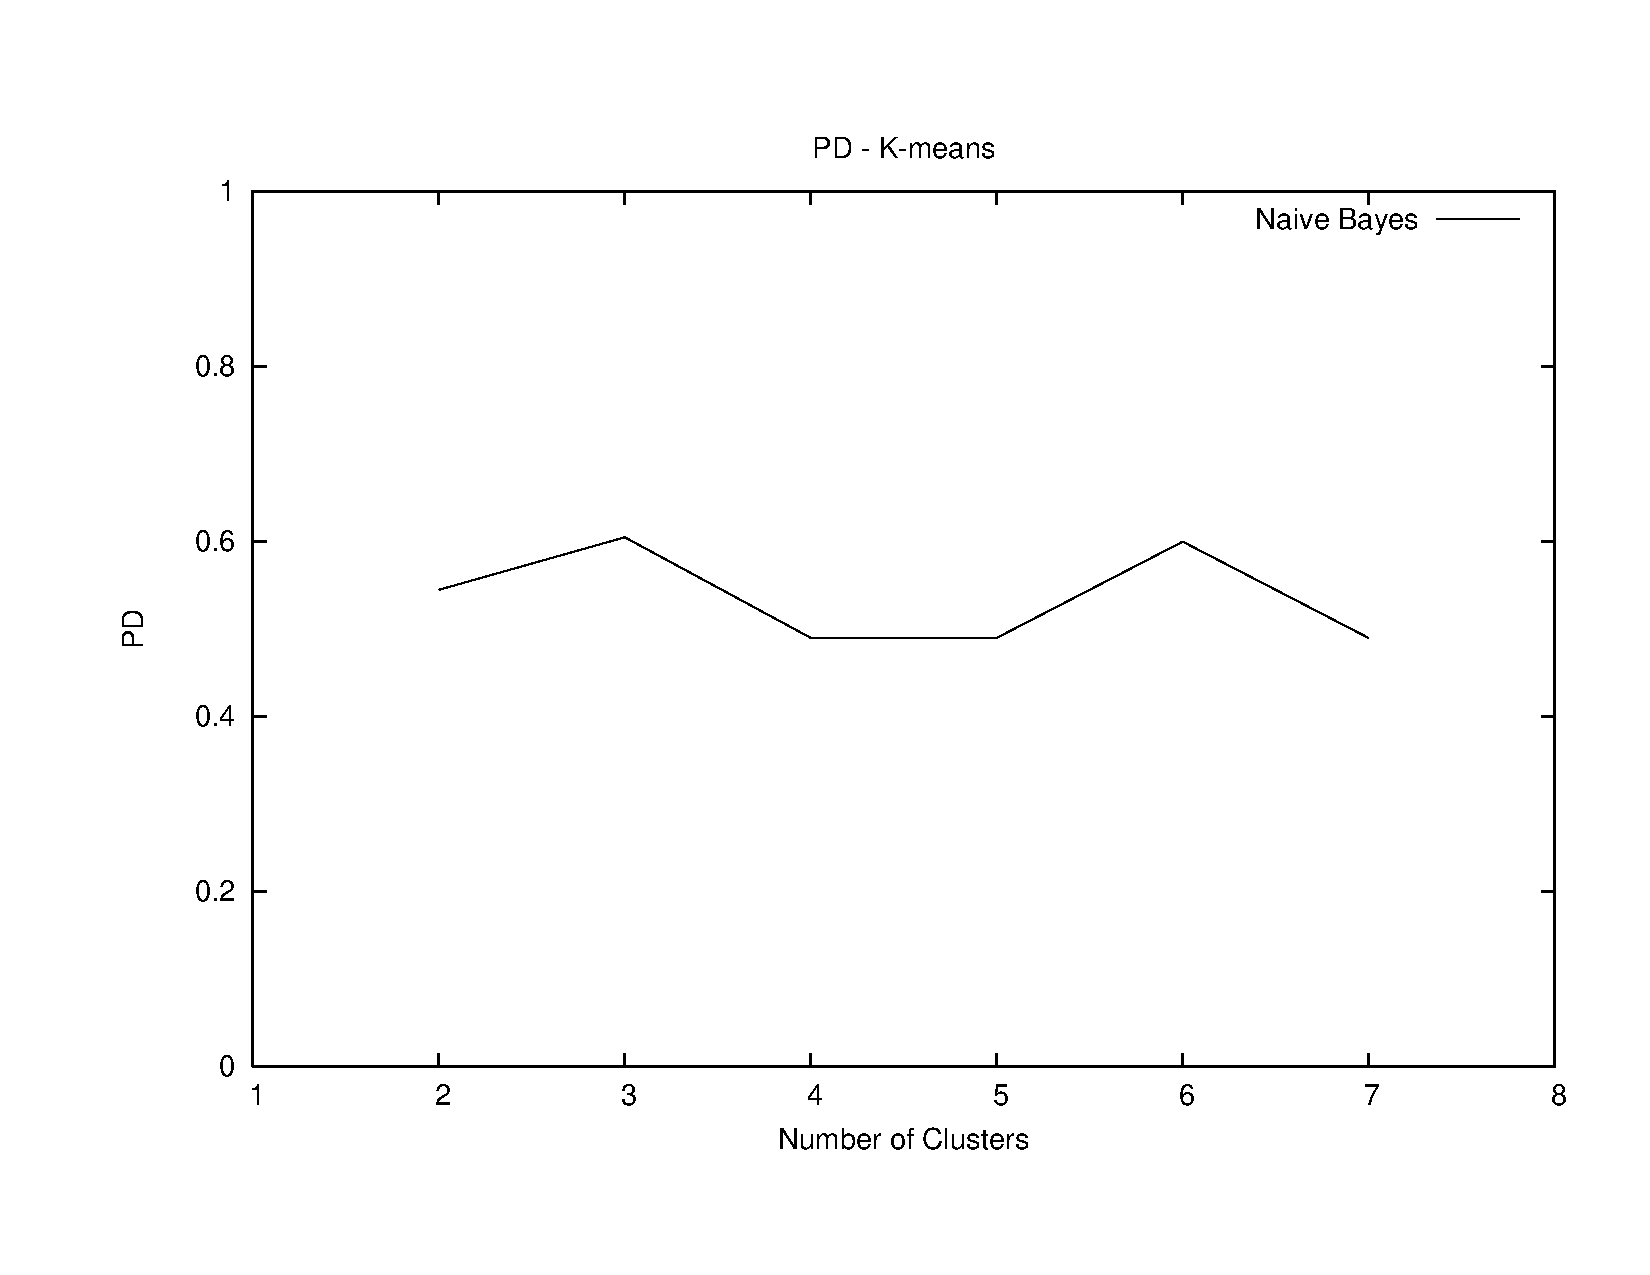
\includegraphics[width=3.5in]{no_disc_nb_cluster_pd.pdf}
  \end{center}

  \caption{\small Figure 1. PD: Naive-Bayes without discretization}
  \label{fig-label}
\end{figure}

\textbf
\begin
  \begin{center}
    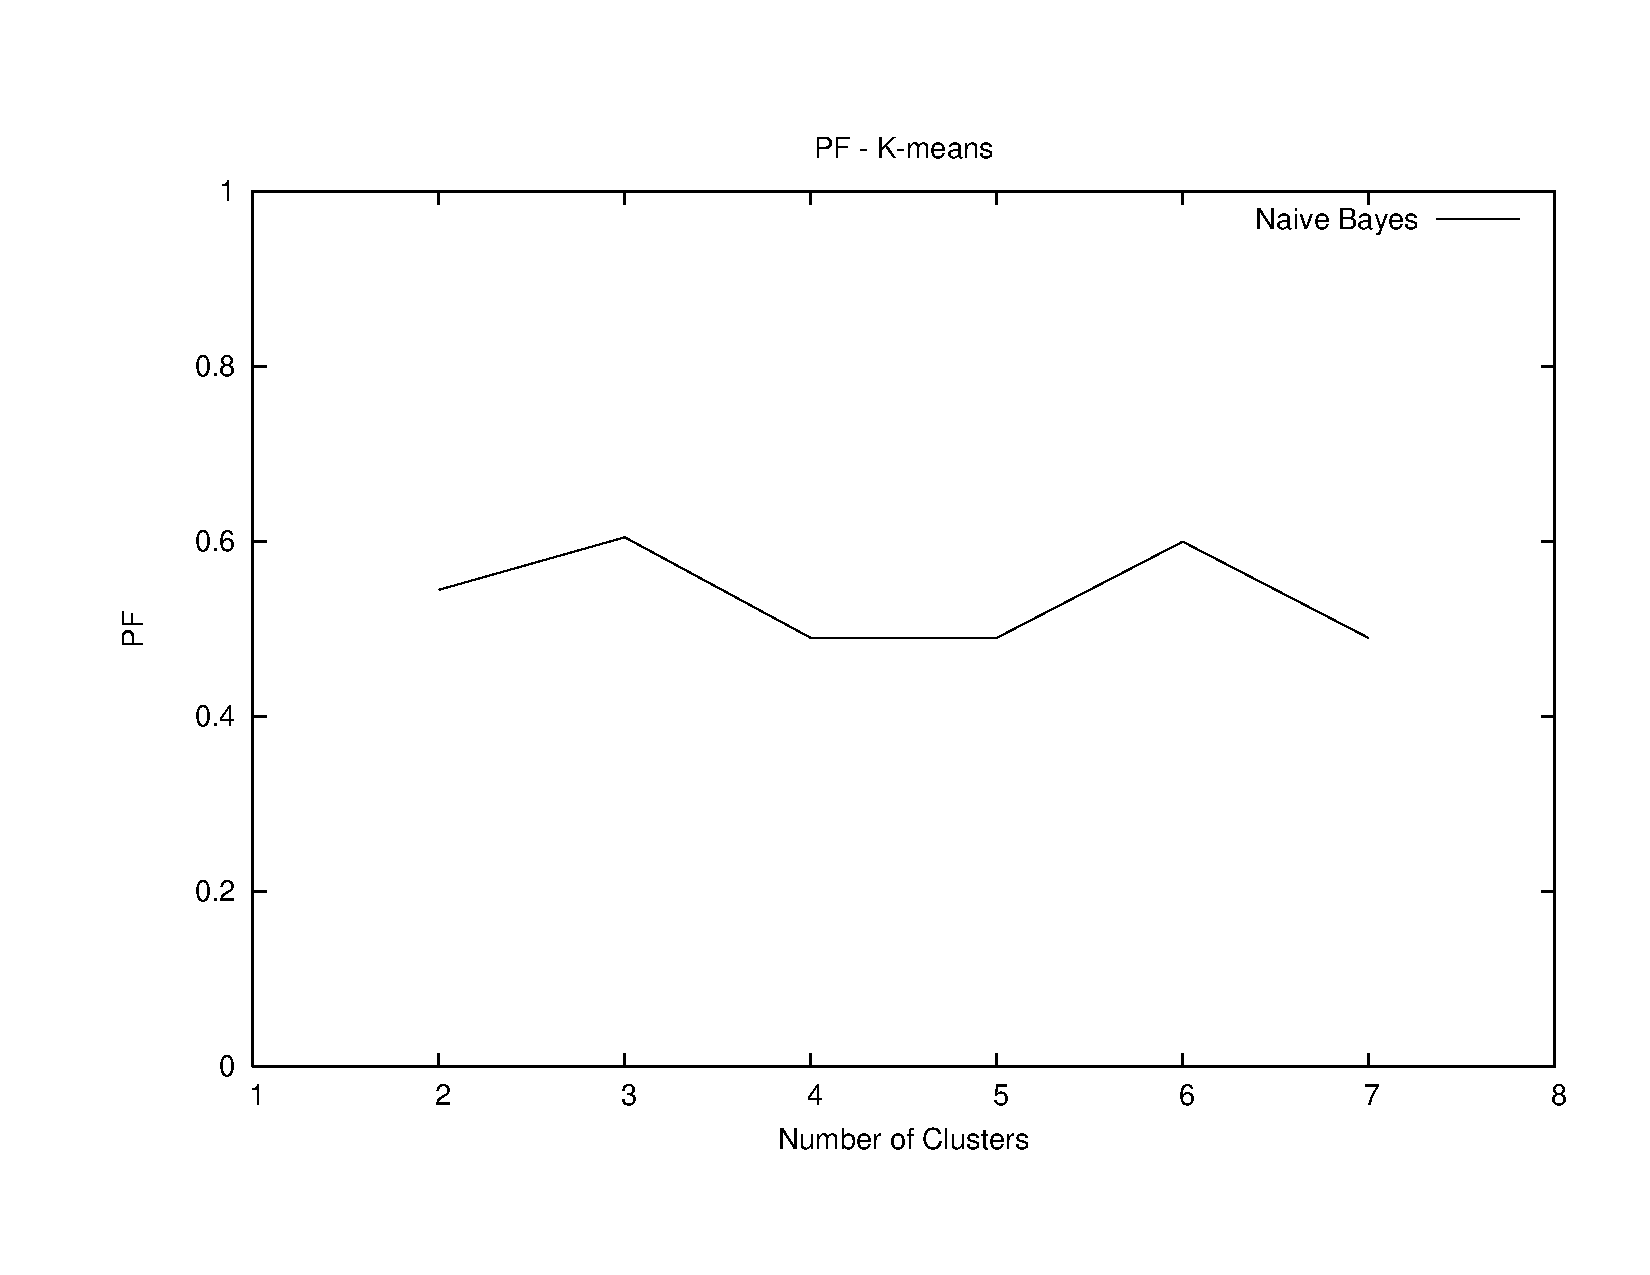
\includegraphics[width=3.5in]{no_disc_nb_cluster_pf.pdf}
  \end{center}

  \caption{\small Figure 2. PF: Naive-Bayes without discretization}
  \label{fig-label} \end{fig-label}
\end{figure}

PD and PF are ploted agains the number of clusters k. Without discretization Naive-Bayes does not perform well. PD is no higher than 60 \%. The number of clusters computed by k-means does not seem to influence the prediction probability however a relatively better PD are retrieved with 3 and 6 number of  clusters. This results also corresponds with \cite {dough95} which state that discretization influence Naive-Bayes performance.
\\
Applying InfoGain on discretize data outperforms the first learner. Data is discretized and InfoGain is used to extract the best n features (columns) from the data. Than Naive-Bayes is applyed on the closest cluster of each instance in the train set.Figure 3 and 4 show the PD and PF of this learner.

 \textbf
\begin
  \begin{center}
    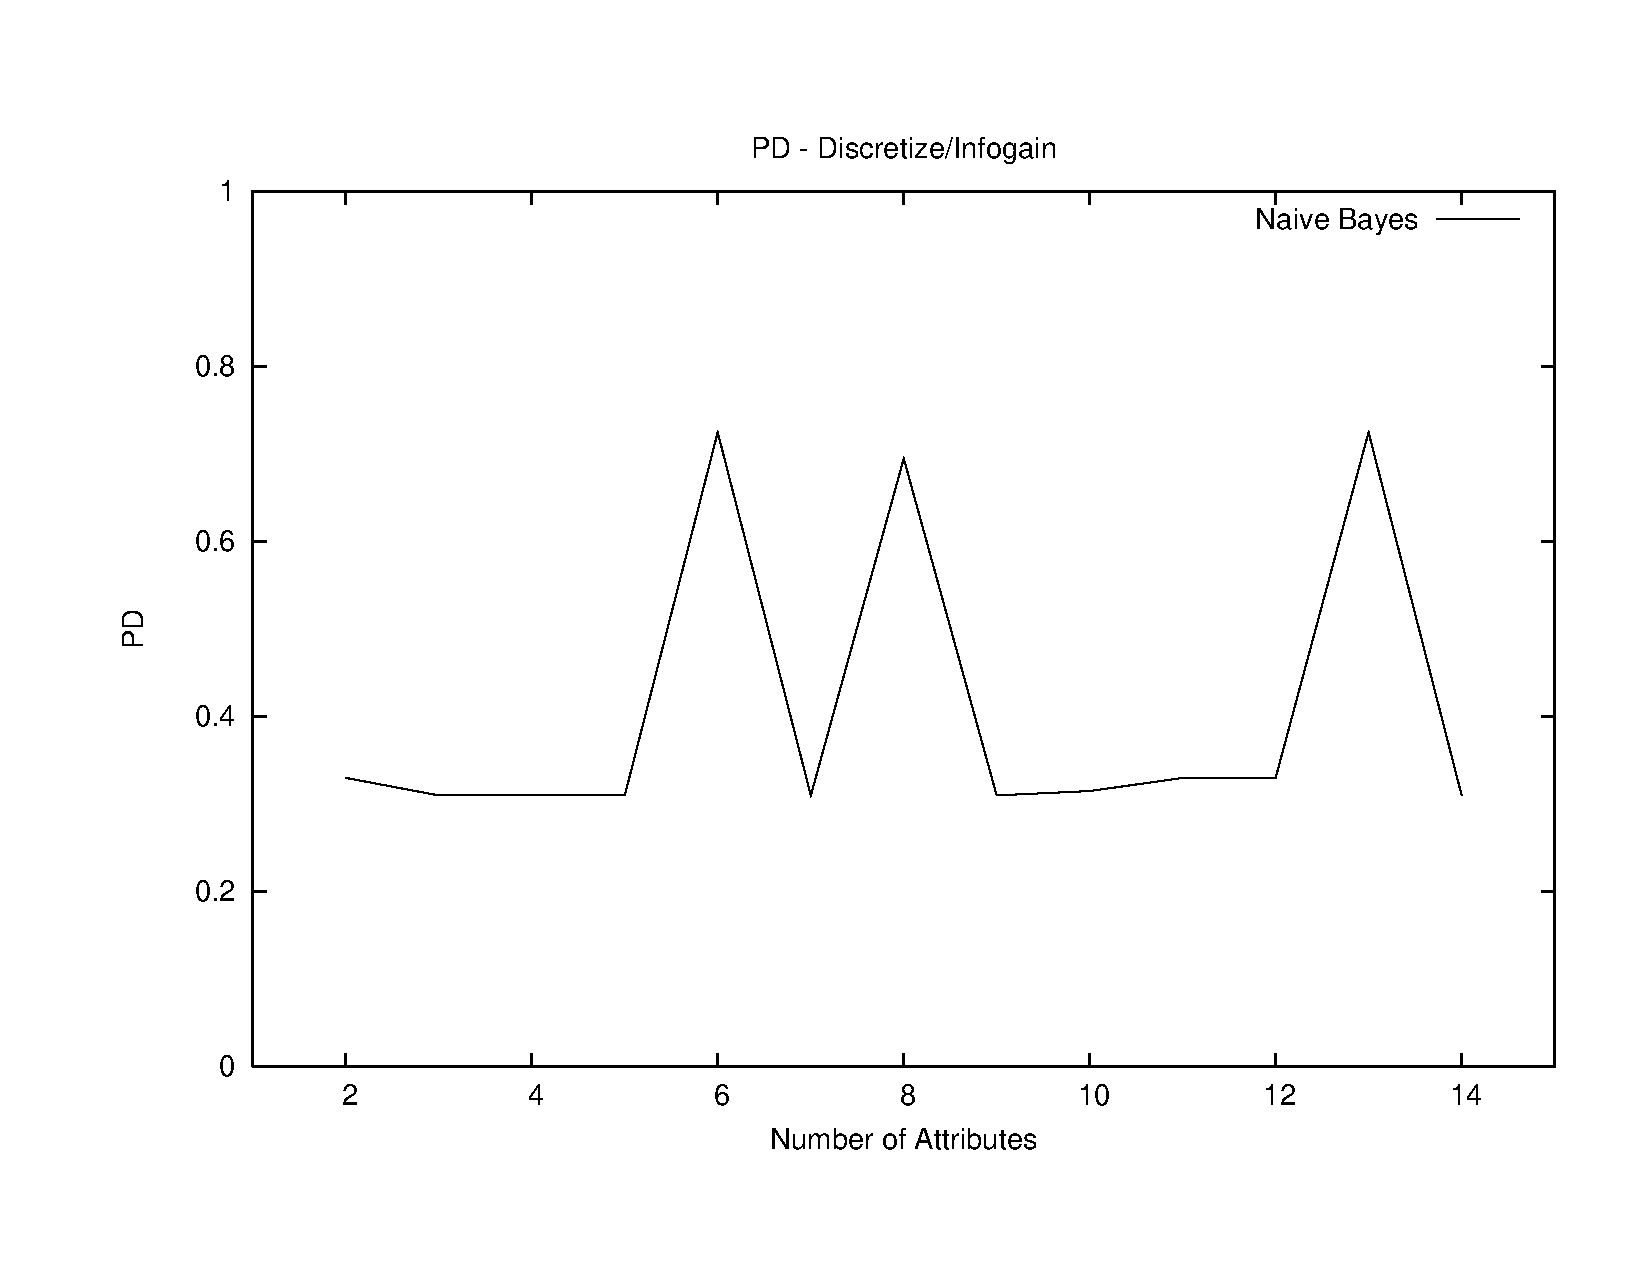
\includegraphics[width=3.5in]{disc_info_pd.pdf}
  \end{center}

  \caption{\small Figure 3. PD: InfoGain and Naive-Bayes}
  \label{fig-label} \end{fig-label}
\end{figure}

\\
\\The second learner scores the highest values for PD when the number of attributes selected by InfoGain n is 6 & 8 and 13. The max PD values are close to 80 \%. In this case the advantage of discretizing the data and applying feature subset selection gives better results than applying the clustering on undiscretized data. 
\textbf
\begin
  \begin{center}
    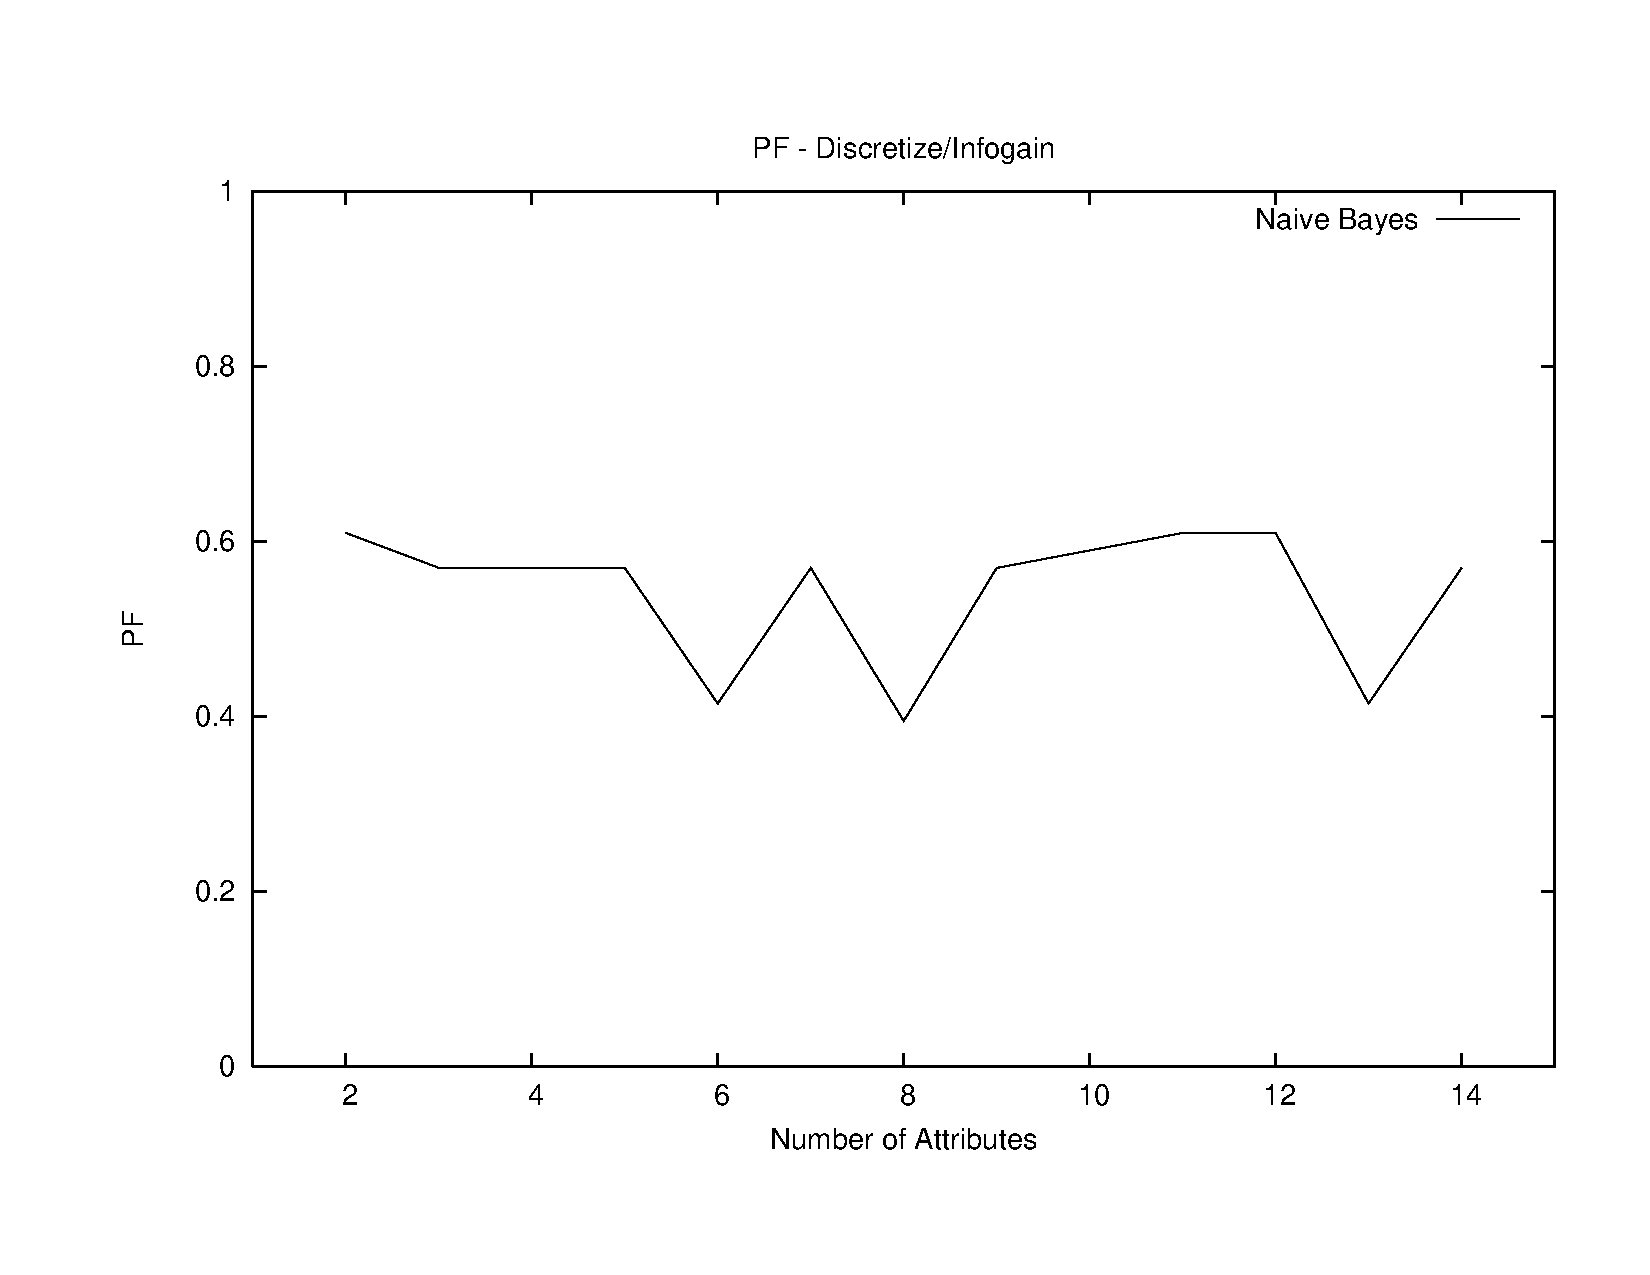
\includegraphics[width=3.5in]{disc_info_pf.pdf}
  \end{center}
  \caption{\small Figure 4. PF InfoGain and Naive-Bayes}
  \label{fig-label} \end{fig-label}
\end{figure}

\\The third learner uses the information supplied by InfoGain to build a new data set containing only the features suggested by InfoGain. Discretization clustering is performed on the data using k-means and Naive-Bayes is trained on each cluster. This learner is exploring a combination of n-features and k-clusters in order to find the optimal solution. Figures 5 and 6 shows the PD and PF for the third learner.
 
\textbf
\begin
  \begin{center}
    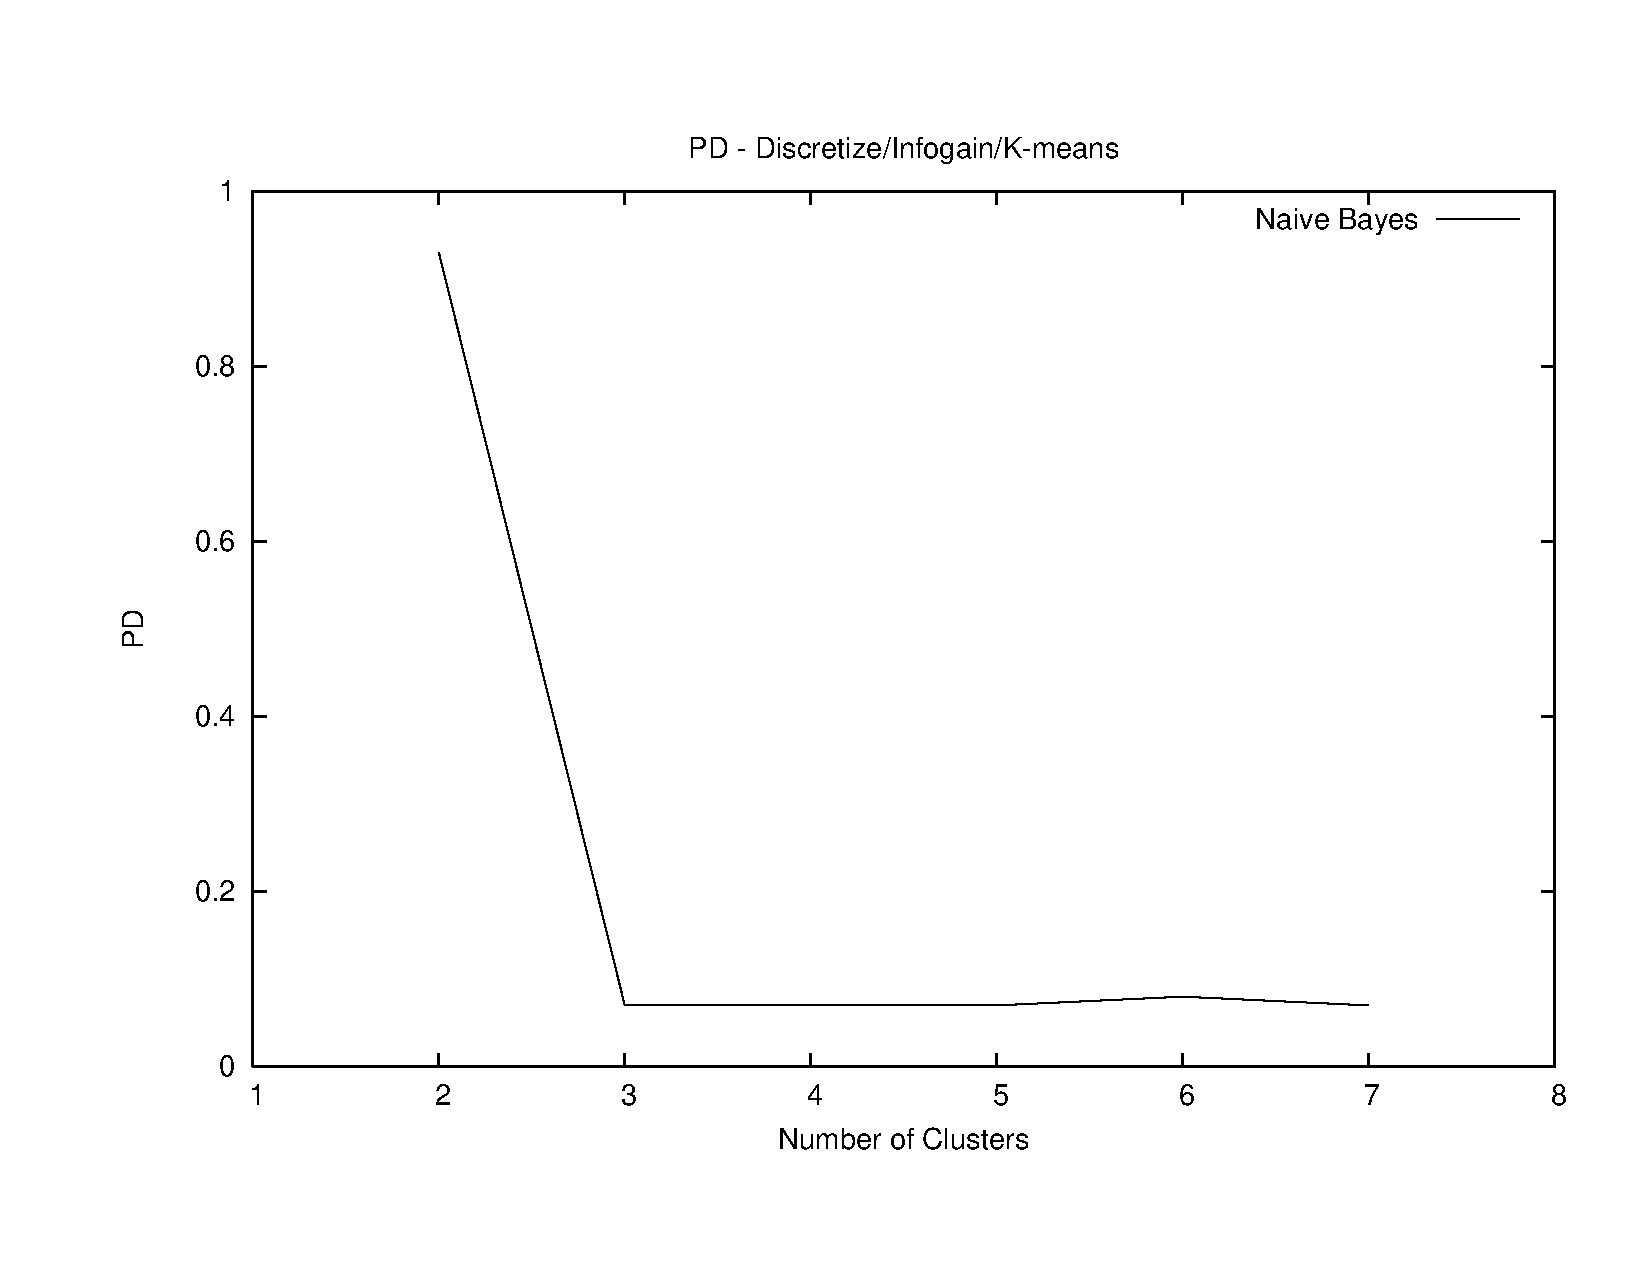
\includegraphics[width=3.5in]{disc_info_cluster_pd.pdf}
  \end{center}
  \caption{\small Figure 5. PD InfoGain/Clustering and Naive-Bayes}
  \label{fig-label} \end{fig-label}
\end{figure}

\textbf
\begin
  \begin{center}
    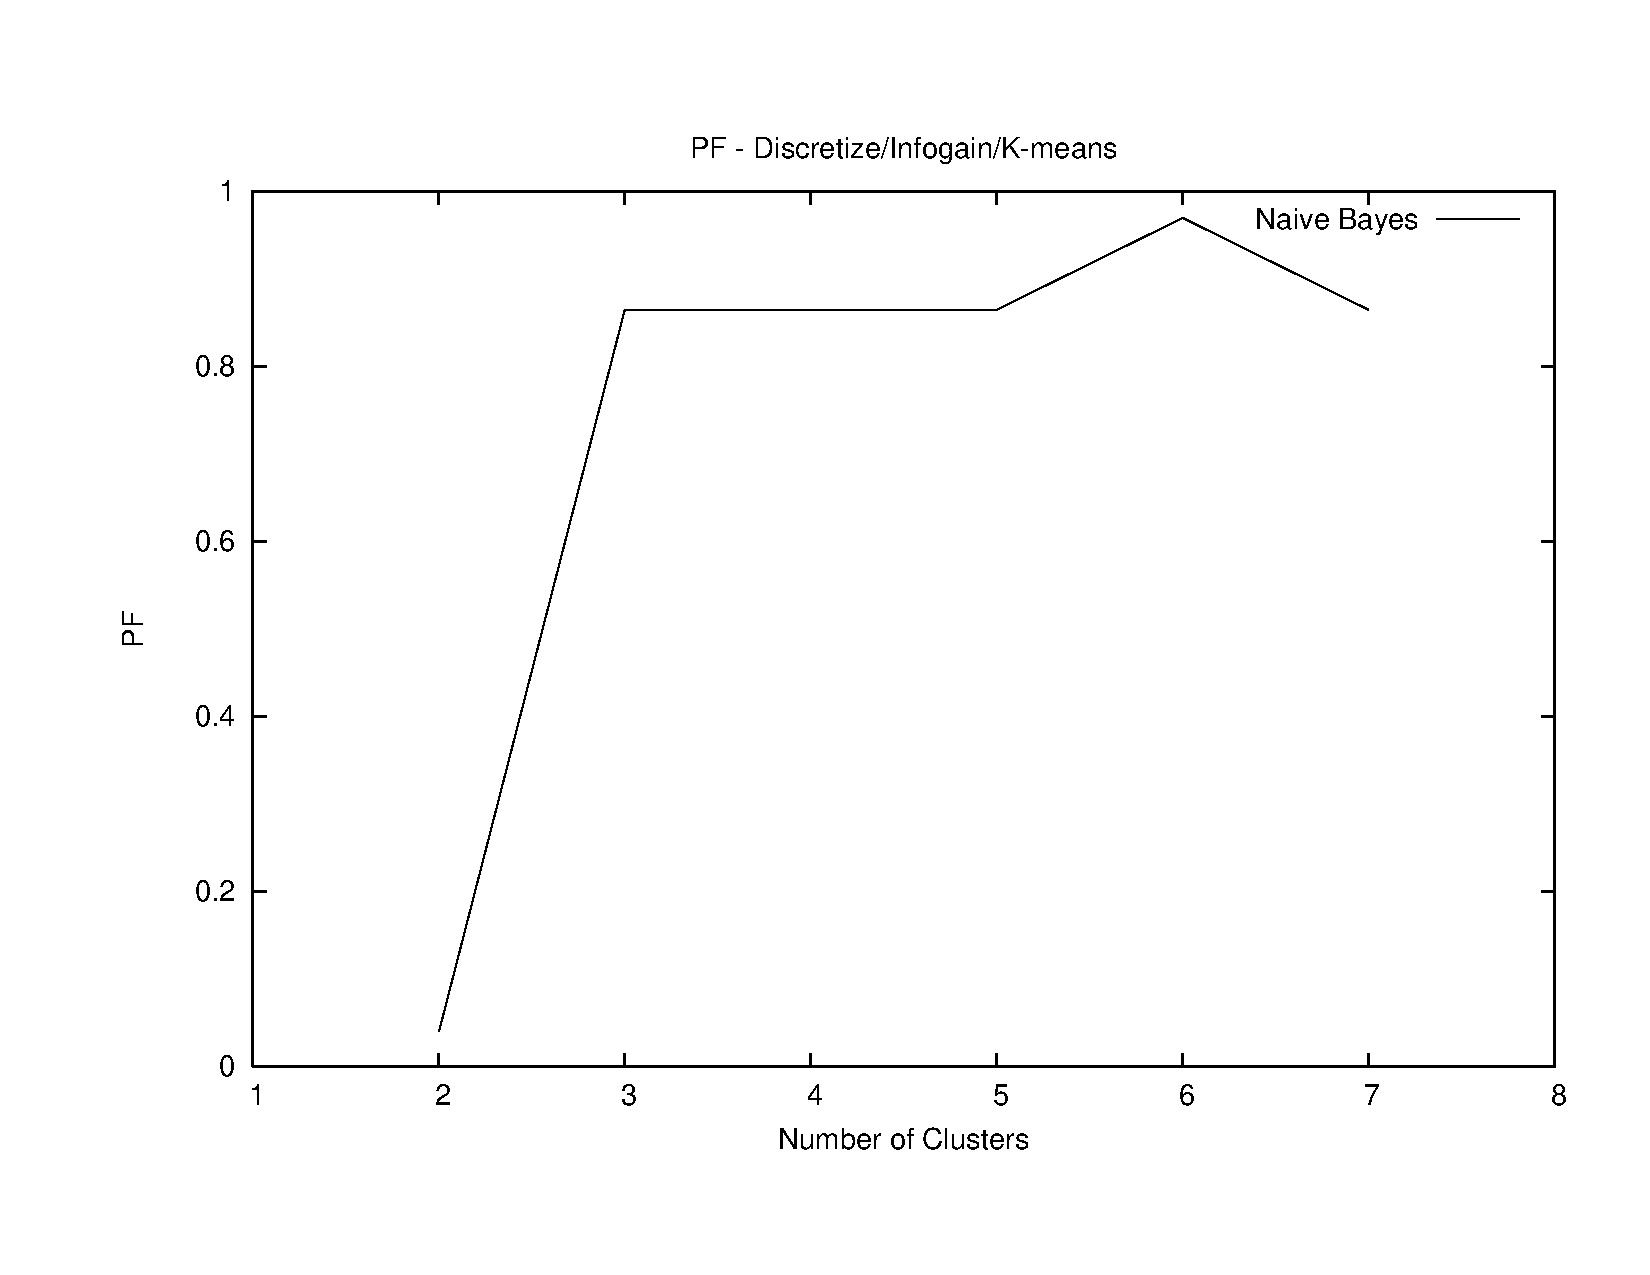
\includegraphics[width=3.5in]{disc_info_cluster_pf.pdf}
  \end{center}
  \caption{\small Figure 6. PF InfoGain/Clustering and Naive-Bayes}
  \label{fig-label} \end{fig-label}
\end{figure}

\\The figures show PD and PF plotted against k-number of clusters which varies from 2 to 7. The PD values decrease sharply when 3 or more clusters are used. The PD remain unchanged as the number of clusters increases. The PD values are relatively high (more than 90 \%) when using less then 3 clusters. These high results should be confirmed by performing further testing as to verify the validity of this approach. 
\\Table 1 . Shows the median PD and PF values for the above three approaches

\begin{table}
\centering
\caption{Statistics for each method}
\begin{tabular}{|c|c|c|c|} \hline
 &PD&PF&Balance\\\hline
No-Discretization-NB& 0.57 & 0.47 & 0.42 \\ \hline
Discretize-Infogain-NB& 0.86 & 0.09 & 0.21 \\ \hline
Infogain-Clustering-NB& 0.5  &0.5  & 0.41 \\ \hline
\end{tabular}
\end{table}

\\Table  2. Shows the top 13 columns selected by InfoGain

\begin{table}
\centering
\caption{Top Features selected by InfoGain}
\begin{tabular}{|c|c|c|c|} \hline
Feat.&Shared_PC1&Shared_CN1&Shared_MW1\\\hline
1& LOComment & I & L\\ \hline
2& LOCCodeAndComment & Uniq-Op & Uniq Opnd\\ \hline
3& Uniq-Opnd & Uniq-Opnd & LOC\\ \hline
4&  I & L & LOComment\\ \hline
5& Uniq-Op & LOComment & LOCCodeAndComment\\ \hline
6& Total-Opnd & LOC & I\\ \hline
7& LOC & Total-Op & BranchCount\\ \hline
8& V & Total-Opnd & V(G)\\ \hline
9& Total-Op & B & V\\ \hline
10& B & V & B\\ \hline
11& LOCode & IV(G) & EV(G)\\ \hline
12& BranchCount & D & LOCode\\ \hline
13& L & BranchCount & Total-Op\\ \hline

\hline\end{tabular}
\end{table}


\section{Related Work}
This project is inspired by the Cross-project Defect Prediction work conducted by Thomas Zimmerman et. al. who claimed that software defect prediction works well whenever there is sufficient data to train any models and that in the case where data is insufficient, cross-project defect prediction suffices\cite{zimmerman09}. In their experiment, they ran 622 cross-project predictions for 12 real-world applications including Microsoft's Internet Explorer and Mozilla Foundation's Firefox web browser, and their results indicated that simply using models from projects in the same domain or with the same process does not lead to accurate predictions. With respect to the experiments they conducted, they learned that Firefox could predict defects in Internet Explorer but not vice versa and they succumbed to the conclusion that this is so because Firefox has more files than Internet Explorer has binaries and that the probability of a software with more data is more likely to predict defects in software with relatively less amount of data or modules. 

Their study led to conclusions that some attributes were less significant than others which is somewhat obvious but also lead to questions such as why defect-prediction is not transivitve. As in, with regards to the experiments they conducted, File system predicted defects in Printing and Printing predicted Clustering but File system did not predict Clustering.

\newpage
\section{Conclusions}
The study undertaken and discussed in this paper involves investigating a criteria for predicting default-prone modules in both small and large-scale software systems. From the experiments performed on each of the data sets we obtained from NASA and SoftLab, we learned that within-company software defect prediction works when the data accumulated for prior versions of the software in question is available. The results from our self-test experiments validates this conclusion. In other words, creating train and test data from the same data set allows us to successfully build models for software defect prediction. This is especially feasible in cases where the company (whose datasets are being used in the experiment) has been around for years, for example NASA, Microsoft or the Mozilla Foundation; or older versions of its software have already been in use for years. The data generated from such older versions can be analyzed, learned on and used to build defect prediction models in order to predict defects in newer versions of the software.

Some researchers indicate that collecting data from case studies and subjecting it to isolated analysis is not enough because statistics on its own does not provide scientific explanations; and that ``we need compelling and sophisticated theories that have the power to explain the empirical observations''\cite{critique}. However, in our experiments, we ran 10 tests on 10 datasets, each time with a different number of nearest-neighbors and number of columns to be selected via infogain, and despite the fact that these experiments were conducted on randomly selected objects from the different data sets and resulted in inconsistencies in the accuracy of defect predictions, the average probability of detection was relatively high while the probability of false alarm was relatively low. Of course, these values were obtained after intensive analysis on the results from applying learners on our datasets which we pre-processed using a number of machine learning / data mining methods as mentioned in section 3.1.


\section{Future Work}
The experiments for this project were conducted using data obtained from NASA and SoftLab for this project simply because they are 2 complete different companies that operate and function in different ways. 
The National Aeronautics and Space Administration (NASA) is an agency of the United States government that undertakes the nation's projects related to space exploration and SoftLab on the other hand is a research laboratory of computer engineering in Turkey that conducts research on cost and effort estimation, defect estimation/prevention, value based software engineering and software process development and typically writes software controllers for home appliances. It is worthy to note that these 2 companies mentioned have no ties with each other. 

We believe that for better results and much better success rates at predicting software defects, regression algorithms could be applied to the datasets to model the data with the least error. That is, apply the learners to the datasets a number of times and discard arguments to algorithms such as k-nearest neighbor and infogain that germinated less desirable results. Also, the learning algorithms used could be altered to analyze additional data instances added to the data already learned on and determine whether the new data would be benefitial to predicting defects or not. Furthermore, this work could be extended to exploit datasets that comprised of more than 2 classes (TRUE, FALSE) and with multiple class columns (at least 2). Also, for any cross-company software defect prediction to be done, datasets from 2 or more different sources but with with similar columns will be required. In the case of our study, the data from SoftLab contained more metrics than that from NASA. This rendered it difficult to build models by learning on the 2 datasets thus experiment on only within-company.

Nonetheless, a number of other rule-based learners could be used rather than {\em NaiveBayes} as was used for this project. These include, but are not limited to, the {\em PRISM} algorithm which aims at inducing modular classification rules directly from the training set; {\em OneR}, {\em TwoR}, {\em RIPPER}, and even {\em HyperPipes}. Due to the constraint on time, we were unable to experiment on such learners but the outcome of applying each of them on the same datasets we used would be of great value to software engineers / data miners. 

Finally, because all the data sets we used were complete, the alrgorithms used in our experiments didn't account for missing values but in future implementations, this will have to be addressed since ignoring this problem can introduce bias into the models being evaluated and lead to inaccurate data mining conclusions. This can easily be done by either ignoring the entire record, filling in with a global constant (not recommended since most data mining algorithms will regard it as a normal value), filling in with the attribute's mean or median, filling in with the most likely value (using regression, decisino trees, most similar records, etc) or using other attributes to predict the value of the missing data \cite{missingdata}.

%
% The following two commands are all you need in the
% initial runs of your .tex file to
% produce the bibliography for the citations in your paper.
\bibliographystyle{abbrv}
\bibliography{refs}  % sigproc.bib is the name of the Bibliography in this case
% You must have a proper ".bib" file
%  and remember to run:
% latex bibtex latex latex
% to resolve all references
%
% ACM needs 'a single self-contained file'!
%
%APPENDICES are optional
%\balancecolumns

\end{document}
